% ============================================================
%  AES (Rijndael): design, implementation and modes of operation
%  Beamer, "terminal" theme (black & white).
%  Compile with XeLaTeX or LuaLaTeX (twice, for the frame count).
%  On Overleaf: Menu > Settings > Compiler > XeLaTeX (or LuaLaTeX).
% ============================================================
\documentclass[aspectratio=169,10pt]{beamer}
\usetheme{terminal}

\usepackage{amsmath,amssymb}
\usepackage{booktabs}
\usepackage{array}
\usepackage{graphicx}
\usepackage{listings}
\usepackage{appendixnumberbeamer}
\usetikzlibrary{arrows.meta,positioning}

% ---------- theme settings ----------
\terminalfootprefix{AES}
\terminalwindow{AES.c}
\terminalshell{%
  \$ ./AES e 1 in.pdf out.pdf KEY\\
  > key expansion ................ ok\\
  > rounds ....................... 10}

\title[Advanced Encryption Standard]{Advanced Encryption\\Standard (Rijndael)}
\subtitle{Design, implementation and modes of operation}
\author{ARGHA SARDAR}
\institute{IISc}
\date{\today}

% ---------- notation ----------
\newcommand{\xor}{\oplus}
\newcommand{\gm}{\bullet}                       % multiplication in GF(2^8)
\newcommand{\GF}{\mathrm{GF}(2^8)}
\newcommand{\fn}[1]{\mathrm{#1}}
\newcommand{\hx}[1]{\ensuremath{\mathtt{\{#1\}}}}            % hex byte {57}
\newcommand{\hh}[1]{\ensuremath{\mathtt{#1}}}                % hex entry in matrices
\newcommand{\Nr}{N_{r}}
\newcommand{\Nk}{N_{k}}
\newcommand{\Nb}{N_{b}}
\newcommand{\kw}[1]{\textbf{#1}}
\newcommand{\ind}{\hspace*{1.1em}}
\newcommand{\cmt}[1]{\hfill{\scriptsize$\triangleright$\ #1}}

% pseudocode: line numbers + body
\newenvironment{pseudo}{\par\footnotesize\renewcommand{\arraystretch}{1.12}%
  \begin{tabular}{@{}r@{\hspace{5pt}}l@{}}}{\end{tabular}\par}

% ---------- code listings ----------
\lstdefinestyle{aesc}{language=C,
  basicstyle=\ttfamily\fontsize{5.9}{6.9}\selectfont,
  keywordstyle=\bfseries, commentstyle=\itshape, stringstyle=\ttfamily,
  showstringspaces=false, columns=fixed, keepspaces=true, tabsize=2,
  breaklines=true, breakindent=1em, breakautoindent=false,
  postbreak=\raisebox{0ex}[0ex][0ex]{\ensuremath{\hookrightarrow\,}},
  aboveskip=0pt, belowskip=0pt, xleftmargin=0pt, xrightmargin=0pt,
  morekeywords={u8,FILE,__m128i}}
\lstset{style=aesc}
\newcommand{\codesmall}{\lstset{basicstyle=\ttfamily\fontsize{5.5}{6.4}\selectfont}}
\newcommand{\codenormal}{\lstset{basicstyle=\ttfamily\fontsize{5.9}{6.9}\selectfont}}

% section dividers: white on black, with the AES machine on the right
\AtBeginSection[]{%
  {\setbeamercolor{background canvas}{bg=black}
   \begin{frame}[plain,noframenumbering]
     \begin{tikzpicture}[remember picture,overlay]
       \node[anchor=east,inner sep=0pt] at ([xshift=-10mm]current page.east)
         {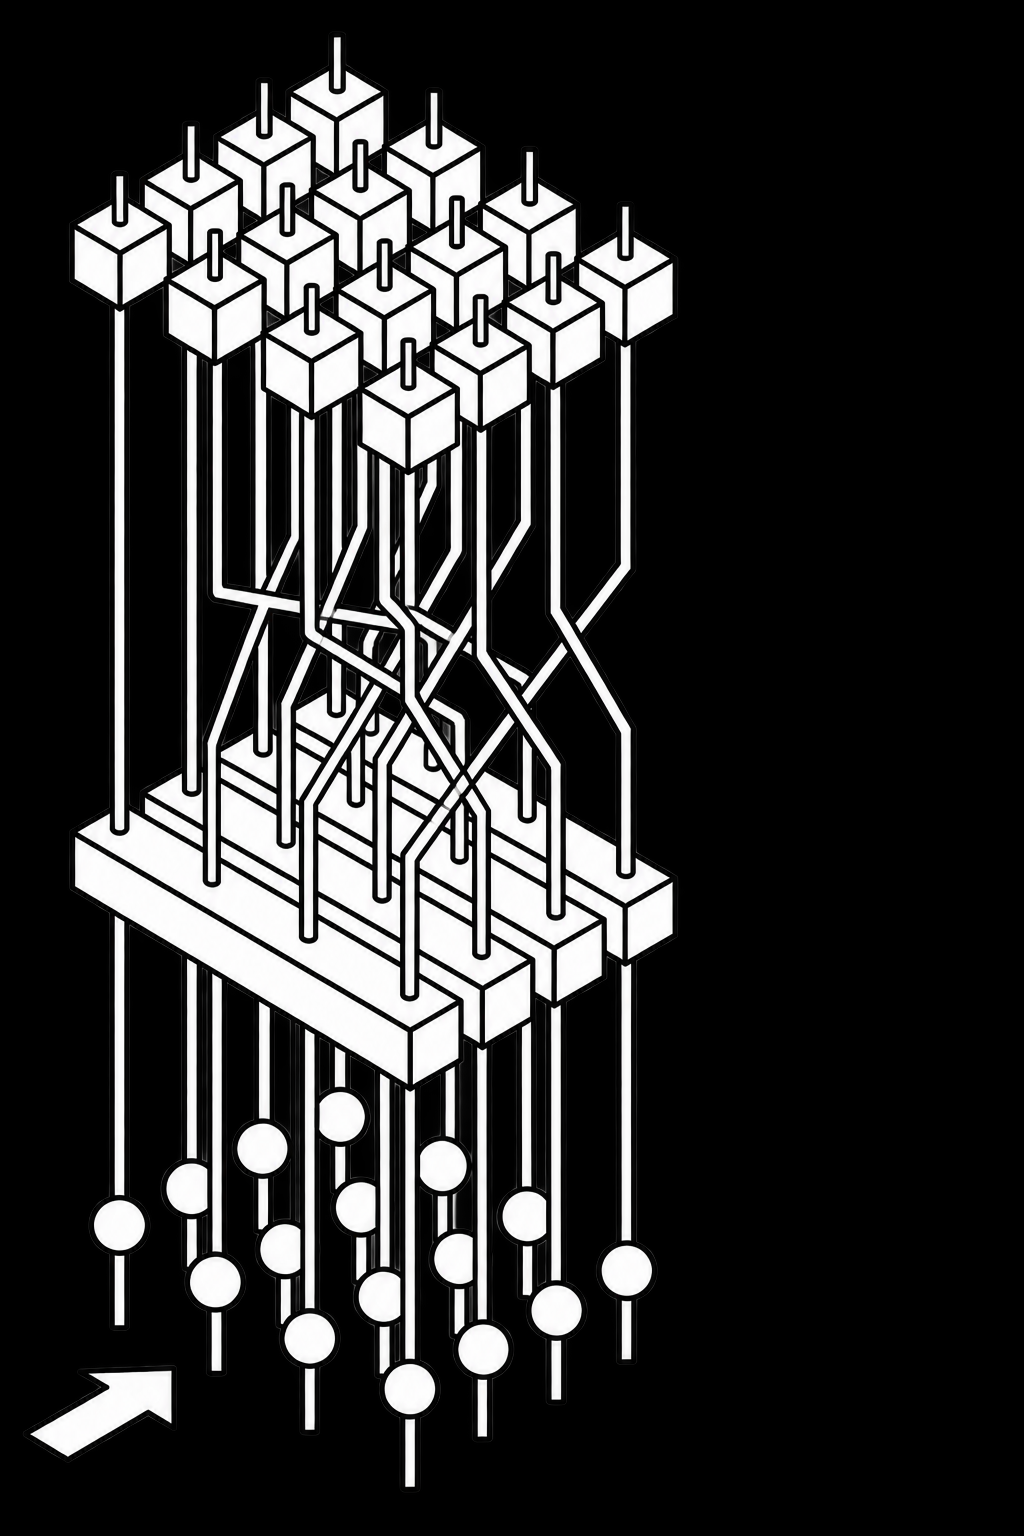
\includegraphics[height=0.66\paperheight]{images/AES_BG.png}};
     \end{tikzpicture}
     \vfill
     \color{white}
     {\small > cd section\_\twod{\value{section}}}\par\vskip10pt
     {\fontsize{40}{44}\selectfont\bfseries \twod{\value{section}}}\par\vskip6pt
     {\LARGE\bfseries \insertsectionhead\,\terminalcursor}\par
     \vfill
   \end{frame}}}

\begin{document}

% ============================================================
%  TITLE
% ============================================================
\begin{frame}[plain,noframenumbering]
\begin{columns}[c]
\begin{column}{0.60\textwidth}
\begin{tcolorbox}[enhanced, sharp corners, colback=white, colframe=black, boxrule=1pt,
  shadow={3pt}{-3pt}{0pt}{fill=black}, left=12pt, right=12pt, top=10pt, bottom=10pt,
  title={\hspace{-4pt}\rule{0.6em}{0.6em}\ \rule{0.6em}{0.6em}\ \rule{0.6em}{0.6em}%
         \hfill AES.c\hfill\phantom{\rule{2.6em}{0.6em}}},
  coltitle=white, colbacktitle=black, fonttitle=\footnotesize\bfseries,
  toptitle=2pt, bottomtitle=2pt, before upper=\raggedright]
\begin{minipage}[c]{0.62\linewidth}
{\Large\bfseries ADVANCED\\ENCRYPTION\\STANDARD\par}
\vskip4pt{\large\bfseries (RIJNDAEL)\par}
\end{minipage}\hfill
\begin{minipage}[c]{0.34\linewidth}\raggedleft

\includegraphics[width=\linewidth]{images/IISc_logo.png}
\end{minipage}
\vskip8pt{\small Design, implementation and\\modes of operation\par}
\vskip12pt{\footnotesize \$ ./AES e 1 in.pdf out.pdf KEY\\
  > key expansion ................ ok\\
  > rounds ....................... 10\ \terminalcursor\par}
\end{tcolorbox}
\end{column}
\begin{column}{0.36\textwidth}
\begin{tbox}[halign=center]{AES round}
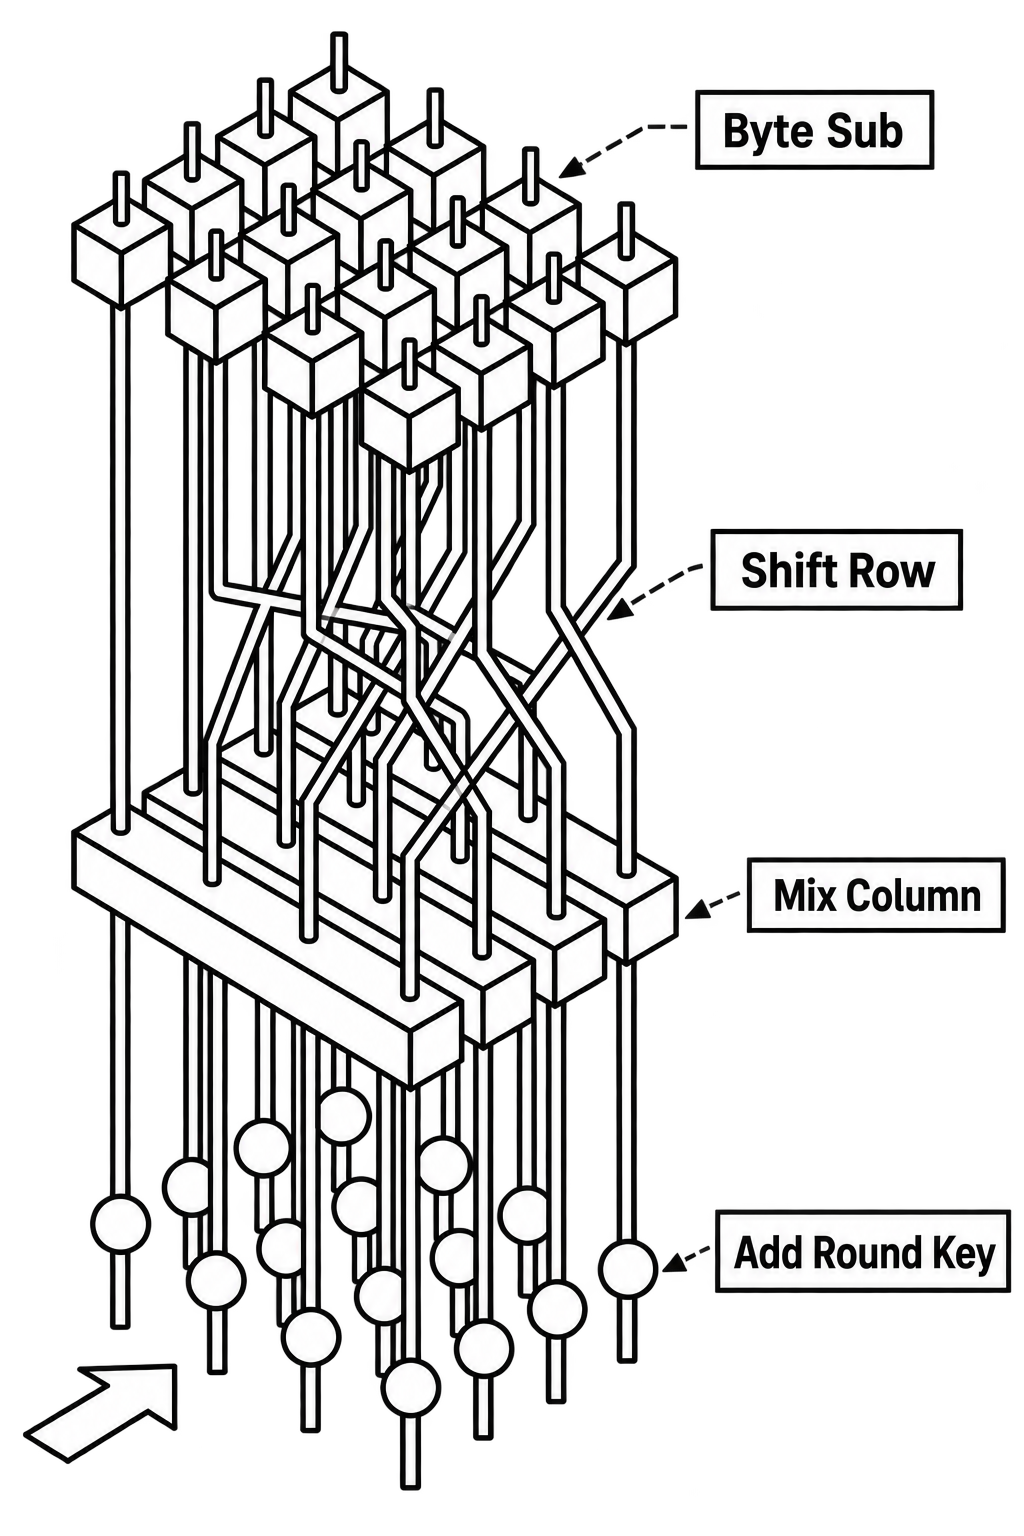
\includegraphics[height=54mm]{images/AES_FRONT.png}\par\vskip5pt
{\small\bfseries ARGHA SARDAR}\par\vskip1pt
{\footnotesize IISc\ \ //\ \ \today}
\end{tbox}
\end{column}
\end{columns}
\end{frame}

% ============================================================
\begin{frame}{Agenda}
\begin{tbox}{> ls talk/}
\small
\begin{tabular}{@{}l@{\quad}l@{}}
01 & introduction: block ciphers, history, parameters \\
02 & preliminaries: the state, arithmetic in $\GF$, the S-box \\
03 & encryption: SubBytes, ShiftRows, MixColumns, AddRoundKey, KeyExpansion \\
04 & decryption: InvCipher and the equivalent inverse cipher \\
05 & look-up table implementation (T-tables) \\
06 & modes of operation: ECB, CBC, OFB, CTR \\
07 & our C implementation and references \\
\end{tabular}
\end{tbox}
\vskip6pt
\footnotesize Notation follows FIPS~197: state $s_{r,c}$, round count $\Nr$, key words $\Nk$, $\Nb=4$,
transformed values are primed ($s'$), $\xor$ is XOR, $\gm$ is multiplication in $\GF$.
\end{frame}

% ============================================================
\section{INTRODUCTION}

\begin{frame}{Block ciphers}
\begin{columns}[T]
\begin{column}{0.55\textwidth}
\begin{itemize}
\item A \alert{block} is a bit sequence of fixed length $n$.
\item A \alert{block cipher} is a map
  \[ E:\ \mathcal{K}\times\{0,1\}^{n}\to\{0,1\}^{n}, \]
  such that for every $K\in\mathcal{K}$ the function $E_K(\cdot)\triangleq E(K,\cdot)$
  is a \alert{bijection} of $\{0,1\}^{n}$.
\item Decryption is the inverse permutation: $D_K=E_K^{-1}$.
\item A block cipher is a fundamental primitive and the basis of services
  that provide \alert{confidentiality} (via modes of operation, Sec.~06).
\end{itemize}
\end{column}
\begin{column}{0.42\textwidth}
\begin{tbox}{AES as a block cipher}
\small
$n=128$ bits (16 bytes)\\[2pt]
$|K|\in\{128,192,256\}$ bits\\[2pt]
$E_K=\fn{Cipher}(\cdot,\Nr,\fn{KeyExpansion}(K))$\\[4pt]
$\fn{Cipher}$ is a permutation of $\{0,1\}^{128}$ for each key;
$\fn{InvCipher}$ is its inverse.
\end{tbox}
\end{column}
\end{columns}
\src{Rijndael AES Implementation \S1; FIPS 197 \S3.1, \S5}
\end{frame}

\begin{frame}{History of AES (1/2): the competition}
\footnotesize
\renewcommand{\arraystretch}{1.18}
\begin{tabular}{@{}>{\bfseries}p{2.3cm}p{9.3cm}@{}}
\toprule
2 Jan 1997 & NIST announces the search for an unclassified, publicly disclosed successor to DES (published 1977). \\
12 Sep 1997 & Formal call: block ciphers with 128-bit blocks and 128/192/256-bit keys. \\
1998 & 15 designs submitted (incl.\ MARS, RC6, Rijndael, Serpent, Twofish); conferences AES1 (Aug 1998), AES2 (Mar 1999). \\
Aug 1999 & Five finalists: \textbf{MARS, RC6, Rijndael, Serpent, Twofish}. \\
3 Sep 1999 & Daemen and Rijmen (Belgium) submit ``AES Proposal: Rijndael'', derived from the Square cipher. \\
Apr 2000 & AES3 conference: finalist teams present, then a vote. \\
2 Oct 2000 & NIST announces \textbf{Rijndael} as the proposed AES. \\
\bottomrule
\end{tabular}
\src{Wikipedia: ``Advanced Encryption Standard'' and ``AES process''; Rijndael AES Implementation \S1}
\end{frame}

\begin{frame}{History of AES (2/2): standard and cryptanalysis}
\footnotesize
\renewcommand{\arraystretch}{1.18}
\begin{tabular}{@{}>{\bfseries}p{2.3cm}p{9.3cm}@{}}
\toprule
26 Nov 2001 & Published as \textbf{FIPS PUB 197}; effective as a US federal standard 26 May 2002; later ISO/IEC 18033-3. \\
Jun 2003 & Approved for US government information up to SECRET (all key sizes); TOP SECRET needs 192/256-bit keys. \\
2005--2010 & Cache-timing attacks on table-based software (Bernstein 2005; Osvik--Shamir--Tromer); Intel AES-NI hardware instructions (2010). \\
2009--2011 & Related-key attacks on AES-192/256 (not on the full cipher as used); first key recovery on full AES by biclique attack (Bogdanov--Khovratovich--Rechberger 2011): $2^{126.2}$ for AES-128, about $4\times$ faster than brute force. \\
2015 & Tao--Wu improve it to $2^{126.0}$, $2^{189.9}$, $2^{254.3}$ (AES-128/192/256). \\
9 May 2023 & FIPS 197 updated (update 1). \\
\bottomrule
\end{tabular}
\vskip4pt
\begin{ibox}\small No practical attack is known against correctly implemented AES.\end{ibox}
\src{Wikipedia: ``Advanced Encryption Standard''; FIPS 197; Rijndael AES Implementation \S5.1, \S5.4}
\end{frame}

\begin{frame}[fragile]{AES parameters}
\begin{columns}[T]
\begin{column}{0.52\textwidth}
\centering\footnotesize
\begin{tabular}{@{}lrrrr@{}}
\toprule
 & $\Nk$ & key bits & $\Nb$ & $\Nr$ \\
\midrule
AES-128 & 4 & 128 & 4 & \textbf{10} \\
AES-192 & 6 & 192 & 4 & 12 \\
AES-256 & 8 & 256 & 4 & 14 \\
\bottomrule
\end{tabular}
\vskip8pt
\raggedright\small
\begin{align*}
\fn{AES\text{-}}k(\mathit{in},\mathit{key}) &= \fn{Cipher}(\mathit{in},\Nr,\fn{KeyExpansion}(\mathit{key}))
\end{align*}
\begin{itemize}\footnotesize
\item Key schedule: $4(\Nr+1)$ words $w[i]$.
\item AES-128 needs $4\cdot 11=44$ words $=176$ bytes.
\item Our implementation: \alert{AES-128 only}.
\end{itemize}
\end{column}
\begin{column}{0.46\textwidth}
%CODE utils.h
\begin{tbox}{utils.h}
\begin{lstlisting}
#define NK 4  // Number of 32-bit words
              // in the key (AES-128: Nk=4)
#define NR 10 // Number of rounds
              // (AES-128: Nr=10)
typedef unsigned char u8;
void KeyExpansion(u8* key, u8* w);
void Cipher(u8* state, u8* ExpandedKey);
...
void InvCipher( u8* state, u8* ExpandedKey);
\end{lstlisting}
\end{tbox}
\vskip4pt
%CODE AES.c
\begin{tbox}{AES.c}
\begin{lstlisting}
u8 key[16];
...
u8 ExpandedKey[176];
KeyExpansion(key, ExpandedKey);
\end{lstlisting}
\end{tbox}
\end{column}
\end{columns}
\src{FIPS 197 \S5, Table 3; AESFINAL/utils.h, AES.c}
\end{frame}

% ============================================================
\section{PRELIMINARIES}

\begin{frame}[fragile]{Bytes, the state and words}
\begin{columns}[T]
\begin{column}{0.56\textwidth}
\begin{itemize}\footnotesize
\item Input block $\mathit{in}_0,\dots,\mathit{in}_{15}$ (bytes) is copied into the
  \alert{state} $s$, a $4\times4$ byte array, \alert{column by column}:
  \[ s[r,c]=\mathit{in}[r+4c],\qquad \mathit{out}[r+4c]=s[r,c], \]
  for $0\le r<4,\ 0\le c<4$.
\item A \alert{word} is 4 bytes. Column $c$ of the state is the word
  $v_c=(s_{0,c},s_{1,c},s_{2,c},s_{3,c})^{T}$.
\item The key schedule is an array $w[0..4(\Nr{+}1){-}1]$ of words;
  $w[i..i{+}3]$ denotes four consecutive words.
\end{itemize}
\vskip2pt
\scriptsize\centering
$\begin{array}{|c|c|c|c|}\hline
s_{0,0} & s_{0,1} & s_{0,2} & s_{0,3}\\\hline
s_{1,0} & s_{1,1} & s_{1,2} & s_{1,3}\\\hline
s_{2,0} & s_{2,1} & s_{2,2} & s_{2,3}\\\hline
s_{3,0} & s_{3,1} & s_{3,2} & s_{3,3}\\\hline
\end{array}\ =\
\begin{array}{|c|c|c|c|}\hline
\mathit{in}_0 & \mathit{in}_4 & \mathit{in}_8 & \mathit{in}_{12}\\\hline
\mathit{in}_1 & \mathit{in}_5 & \mathit{in}_9 & \mathit{in}_{13}\\\hline
\mathit{in}_2 & \mathit{in}_6 & \mathit{in}_{10} & \mathit{in}_{14}\\\hline
\mathit{in}_3 & \mathit{in}_7 & \mathit{in}_{11} & \mathit{in}_{15}\\\hline
\end{array}$
\end{column}
\begin{column}{0.41\textwidth}
%CODE utils.h
\begin{tbox}{utils.h}
\begin{lstlisting}
typedef unsigned char u8;
void KeyExpansion(u8* key, u8* w);
void Cipher(u8* state, u8* ExpandedKey);
\end{lstlisting}
\end{tbox}
\vskip4pt
\begin{pbox}\footnotesize
\texttt{u8 state[16]} holds the state in \alert{column-major} order:
$s_{r,c}=\texttt{state}[\,r+4c\,]$.\par\vskip2pt
Column $c$ is the contiguous slice \texttt{state[4c..4c+3]}, which is why
\texttt{MixColumns} works on \texttt{s[0..3]}, \texttt{s[4..7]}, \texttt{s[8..11]}, \texttt{s[12..15]}.\par\vskip2pt
Row $r$ is strided: \texttt{state[r]}, \texttt{state[r+4]}, \texttt{state[r+8]}, \texttt{state[r+12]}.
\end{pbox}
\end{column}
\end{columns}
\src{FIPS 197 \S3.4--3.5, Fig.~1; AESFINAL/utils.h}
\end{frame}

\begin{frame}{Arithmetic in $\GF$: addition and multiplication}
\begin{columns}[T]
\begin{column}{0.50\textwidth}
\begin{tbox}{byte $\leftrightarrow$ polynomial}
\small
$\{b_7b_6\dots b_0\}\ \leftrightarrow\ b(x)=\sum_{i=0}^{7}b_i x^i,\quad b_i\in\mathbb{F}_2$
\end{tbox}
\vskip6pt
\begin{tbox}{addition = XOR}
\small
Coefficients are added mod 2, so $a+b=a\xor b$; addition equals subtraction and $a\xor a=\hx{00}$.\\[3pt]
$\hx{57}\xor\hx{83}=\hx{d4}$\\
$(x^6{+}x^4{+}x^2{+}x{+}1)+(x^7{+}x{+}1)=x^7{+}x^6{+}x^4{+}x^2$
\end{tbox}
\end{column}
\begin{column}{0.47\textwidth}
\begin{tbox}{multiplication}
\small
\[ b\gm c \;=\; b(x)\,c(x)\bmod m(x) \]
with the fixed irreducible polynomial
\[ m(x)=x^8+x^4+x^3+x+1\ \ (\hx{11b}). \]
\end{tbox}
\vskip6pt
\begin{tbox}{inverse}
\small
For $b\neq\hx{00}$ there is a unique $b^{-1}$ with $b\gm b^{-1}=\hx{01}$:
\[ b^{-1}=b^{254}. \]
(or via extended Euclid: $b(x)a(x)+m(x)c(x)=1$).
\end{tbox}
\end{column}
\end{columns}
\src{FIPS 197 \S4.1--4.4; Rijndael AES Implementation \S2.1}
\end{frame}

\begin{frame}[fragile]{xtime: multiplication by $\hx{02}$}
\begin{columns}[T]
\begin{column}{0.54\textwidth}
\small
Multiplying by $x$ shifts the polynomial; reduce by $m(x)$ if the degree reaches 8:
\[ \fn{xtime}(b)=b\gm\hx{02}=
\begin{cases}\{b_6b_5\dots b_0\,0\} & b_7=0\\
\{b_6b_5\dots b_0\,0\}\xor\hx{1b} & b_7=1\end{cases}\]
Any constant is a sum of powers of $\hx{02}$; with $b=\hx{57}$:\\[2pt]
\footnotesize
$\hx{57}\gm\hx{02}=\hx{ae},\ \hx{04}\!:\hx{47},\ \hx{08}\!:\hx{8e},\ \hx{10}\!:\hx{07}$\\[2pt]
$\hx{13}=\hx{10}\xor\hx{02}\xor\hx{01}$, hence\\
$\hx{57}\gm\hx{13}=\hx{57}\xor\hx{ae}\xor\hx{07}=\hx{fe}$\\[2pt]
Horner form for $\hx{15}=\hx{01}\xor\hx{04}\xor\hx{10}$:\\
$b\gm\hx{15}=b\xor\fn{xtime}^2\!\big(b\xor\fn{xtime}^2(b)\big)$
\end{column}
\begin{column}{0.44\textwidth}
%CODE utils.c
\begin{tbox}{utils.c :: xtime (constant time)}
\begin{lstlisting}
// xtime function: multiplies by
// 0x02 in GF(2^8)
u8 xtime(u8 b) {
    return (b << 1) ^ ((b >> 7) * 0x1B);
}
\end{lstlisting}
\end{tbox}
\vskip4pt
\begin{pbox}\footnotesize
Branching version, \alert{data-dependent timing}:\\
\texttt{(b<{}<1) \string^ ((b \& 0x80) ? 0x1B : 0x00)}\\[2pt]
Masking version: $b_7\in\{0,1\}$ times $\hx{1b}$ gives the same value with
\alert{no branch}, so the cycle count is independent of $b$.
\end{pbox}
\end{column}
\end{columns}
\src{FIPS 197 \S4.2 (Eq.~4.5--4.7); Rijndael AES Implementation \S2.1; AESFINAL/utils.c}
\end{frame}

\begin{frame}{The S-box as $f\circ g$: inversion and affine map}
\begin{columns}[T]
\begin{column}{0.47\textwidth}
\small
\[ \fn{SBox}(b)=f\big(g(b)\big) \]
\textbf{1. Inversion} in $\GF$:
\[ g(b)=\tilde b=\begin{cases}\hx{00}& b=\hx{00}\\ b^{-1} & b\neq\hx{00}\end{cases}\]\vskip-4pt
\textbf{2. Affine map}, $c=\hx{63}$, indices mod 8:
\[ b'_i=\tilde b_i\xor\tilde b_{i+4}\xor\tilde b_{i+5}\xor\tilde b_{i+6}\xor\tilde b_{i+7}\xor c_i \]
\end{column}
\begin{column}{0.50\textwidth}
\scriptsize
\[\setlength{\arraycolsep}{2pt}
\begin{bmatrix}b'_0\\b'_1\\b'_2\\b'_3\\b'_4\\b'_5\\b'_6\\b'_7\end{bmatrix}=
\begin{bmatrix}
1&0&0&0&1&1&1&1\\1&1&0&0&0&1&1&1\\1&1&1&0&0&0&1&1\\1&1&1&1&0&0&0&1\\
1&1&1&1&1&0&0&0\\0&1&1&1&1&1&0&0\\0&0&1&1&1&1&1&0\\0&0&0&1&1&1&1&1\end{bmatrix}
\begin{bmatrix}\tilde b_0\\\tilde b_1\\\tilde b_2\\\tilde b_3\\\tilde b_4\\\tilde b_5\\\tilde b_6\\\tilde b_7\end{bmatrix}\xor
\begin{bmatrix}1\\1\\0\\0\\0\\1\\1\\0\end{bmatrix}\]
\end{column}
\end{columns}
\vskip2pt
\begin{itemize}\footnotesize
\item $g$ is non-linear (an involution, $g\circ g=\mathrm{id}$); $f$ is a bijection; so $\fn{SBox}^{-1}=g\circ f^{-1}$.
\item Examples: $\fn{SBox}(\hx{53})=\hx{ed}$, $\fn{SBox}(\hx{00})=\hx{63}$.
\item We use a \alert{256-byte look-up table} for speed (Rijndael AES Implementation \S2.2).
\end{itemize}
\src{FIPS 197 \S5.1.1 (Eq.~5.2--5.4); Rijndael AES Implementation \S2.2}
\end{frame}

% ============================================================
\section{ENCRYPTION}

\begin{frame}{Cipher(): the structure of a round}
\begin{columns}[T]
\begin{column}{0.30\textwidth}
\centering
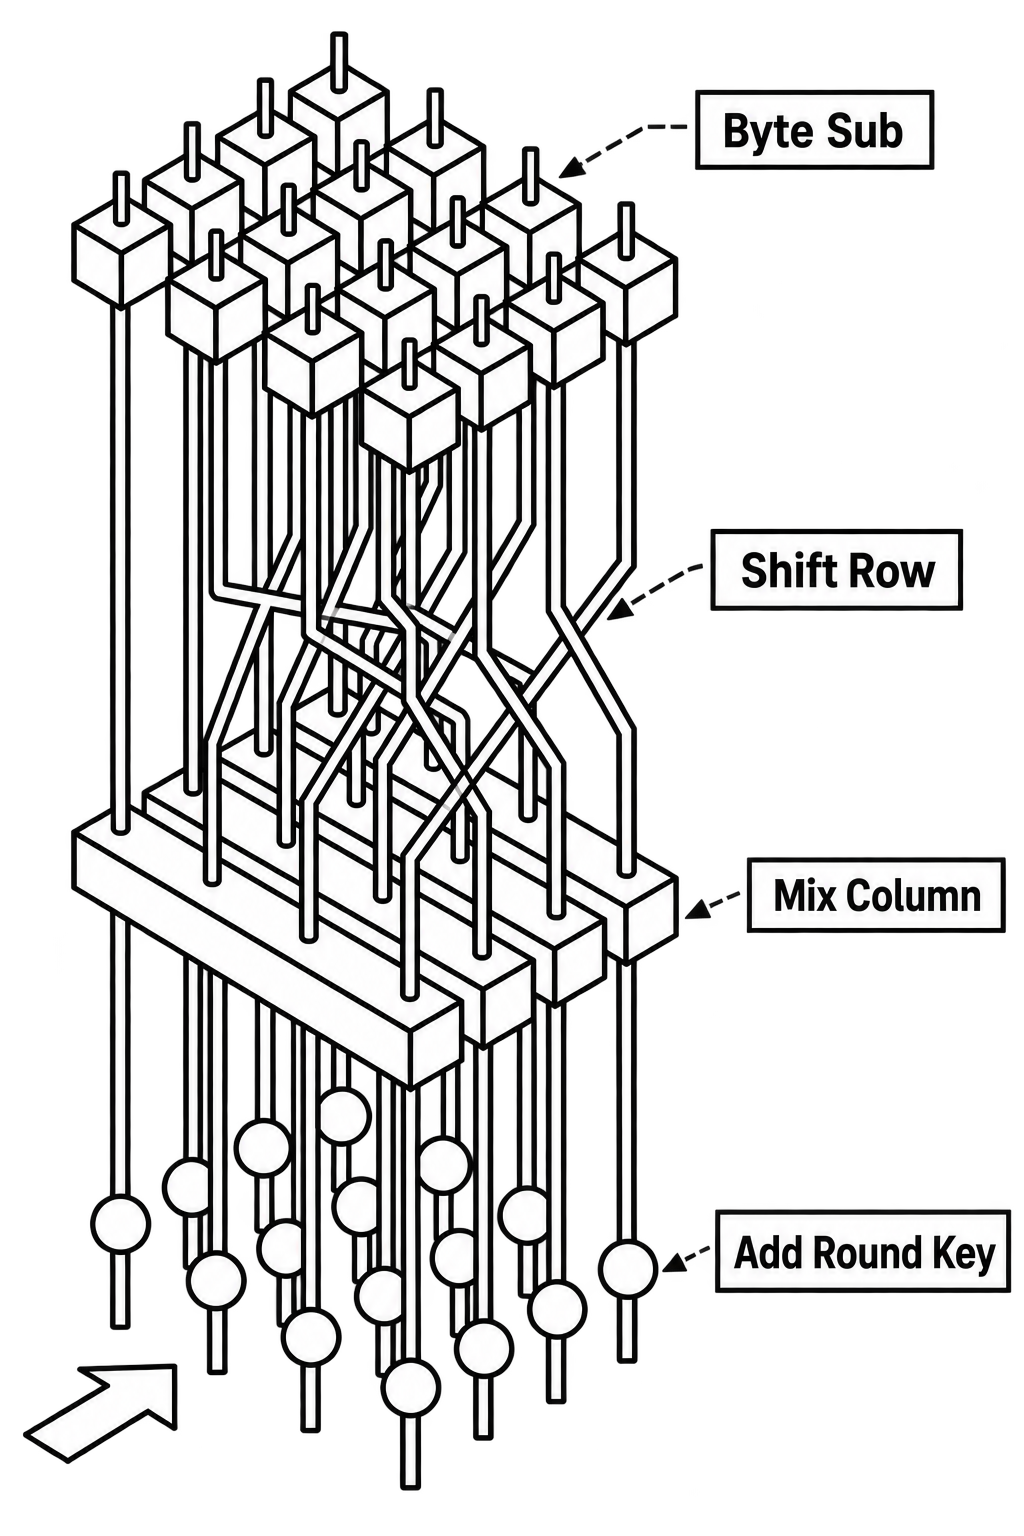
\includegraphics[height=56mm]{images/AES_FRONT.png}
\end{column}
\begin{column}{0.66\textwidth}
\small
Each round applies four byte-oriented transformations to the state:
\begin{enumerate}\footnotesize
\item[\inv{1}] $\fn{SubBytes}$: S-box applied to each of the 16 bytes (non-linear).
\item[\inv{2}] $\fn{ShiftRows}$: row $r$ is rotated left by $r$ positions.
\item[\inv{3}] $\fn{MixColumns}$: each column times a fixed matrix over $\GF$.
\item[\inv{4}] $\fn{AddRoundKey}$: XOR with a 128-bit round key from $\fn{KeyExpansion}$.
\end{enumerate}
\vskip4pt
\begin{tbox}{structure (round index: steps)}
\scriptsize
\begin{tabular}{@{}l@{\ }l@{}}
$0$: & $\fn{AddRoundKey}$ \\
$1..\Nr{-}1$: & $\fn{SubBytes}\to\fn{ShiftRows}\to\fn{MixColumns}\to\fn{AddRoundKey}$ \\
$\Nr$: & $\fn{SubBytes}\to\fn{ShiftRows}\to\fn{AddRoundKey}$ \\
\end{tabular}\\[3pt]
$\Nr+1$ calls of $\fn{AddRoundKey}$; the final round omits $\fn{MixColumns}$.
\end{tbox}
\end{column}
\end{columns}
\src{FIPS 197 \S5.1; figure: Byte Sub / Shift Row / Mix Column / Add Round Key (AES\_FRONT.png)}
\end{frame}

\begin{frame}[fragile]{Cipher(): pseudocode and C}
\begin{columns}[T]
\begin{column}{0.52\textwidth}
\begin{pseudo}
1 & \kw{procedure} \texttt{Cipher}($\mathit{in},\Nr,w$) \\
2 & \ind $\mathit{state}\leftarrow \mathit{in}$ \\
3 & \ind $\mathit{state}\leftarrow\fn{AddRoundKey}(\mathit{state},w[0..3])$ \\
4 & \ind \kw{for} $\mathit{round}=1$ \kw{to} $\Nr-1$ \kw{do} \\
5 & \ind\ind $\mathit{state}\leftarrow\fn{SubBytes}(\mathit{state})$ \\
6 & \ind\ind $\mathit{state}\leftarrow\fn{ShiftRows}(\mathit{state})$ \\
7 & \ind\ind $\mathit{state}\leftarrow\fn{MixColumns}(\mathit{state})$ \\
8 & \ind\ind $\mathit{state}\leftarrow\fn{AddRoundKey}(\mathit{state},$ \\
  & \ind\ind\ind $w[4\,\mathit{round}..4\,\mathit{round}{+}3])$ \\
9 & \ind \kw{end for} \\
10 & \ind $\mathit{state}\leftarrow\fn{SubBytes}(\mathit{state})$ \\
11 & \ind $\mathit{state}\leftarrow\fn{ShiftRows}(\mathit{state})$ \\
12 & \ind $\mathit{state}\leftarrow\fn{AddRoundKey}(\mathit{state},w[4\Nr..4\Nr{+}3])$ \\
13 & \ind \kw{return} $\mathit{state}$ \\
\end{pseudo}
\end{column}
\begin{column}{0.46\textwidth}
%CODE utils.c
\begin{tbox}{utils.c :: Cipher}
\begin{lstlisting}
void Cipher(u8* state, u8* ExpandedKey) {
    // Initial round key addition.
    AddRoundKey(state, ExpandedKey, 0);

    // 9 main rounds.
    for (u8 round = 1; round < NR; ++round) {
        SubBytes(state);
        ShiftRows(state);
        MixColumns(state);
        AddRoundKey(state, ExpandedKey, round);
    }

    // Final round (no MixColumns).
    SubBytes(state);
    ShiftRows(state);
    AddRoundKey(state, ExpandedKey, 10);
}
\end{lstlisting}
\end{tbox}
\end{column}
\end{columns}
\src{FIPS 197 Alg.~1; AESFINAL/utils.c}
\end{frame}

\begin{frame}[fragile]{SubBytes}
\begin{columns}[T]
\begin{column}{0.52\textwidth}
\small
Non-linear, invertible, applied \alert{independently} to every byte:
\[ s'_{r,c}=\fn{SBox}(s_{r,c}),\qquad 0\le r,c<4 \]
\centering
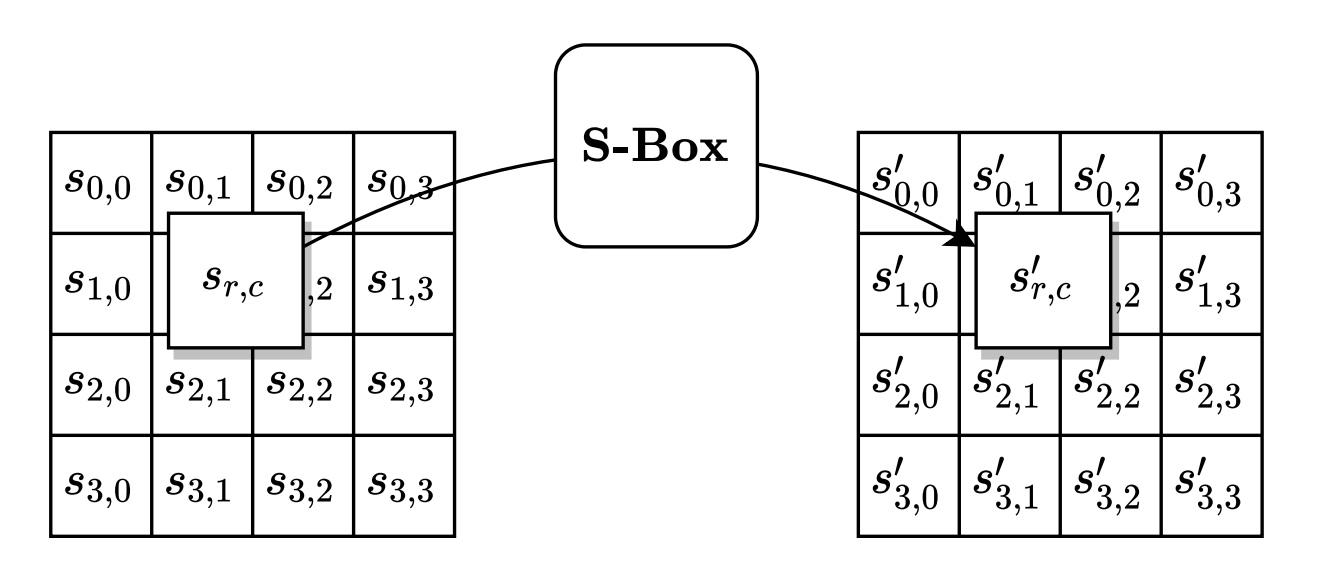
\includegraphics[width=0.95\linewidth]{images/S_Box.png}\par
\raggedright\footnotesize
\begin{itemize}
\item Table: $\fn{SBox}(\{xy\})$ is the entry in row $x$, column $y$.
  E.g.\ $s_{r,c}=\hx{53}\Rightarrow s'_{r,c}=\hx{ed}$.
\item Loop \alert{unrolled}: no loop-control overhead, sequential accesses (better spatial locality and prefetching).
\end{itemize}
\end{column}
\begin{column}{0.45\textwidth}
%CODE utils.c
\begin{tbox}{utils.c :: sbox[256], SubBytes}
\begin{lstlisting}
const u8 sbox[256] = {
    0x63, 0x7c, 0x77, 0x7b, 0xf2, 0x6b,
    0x6f, 0xc5, 0x30, 0x01, 0x67, 0x2b,
    ...
};
\end{lstlisting}
\vskip3pt
\begin{lstlisting}
void SubBytes(u8* state) {
    state[0]  = sbox[state[0]];
    state[1]  = sbox[state[1]];
    state[2]  = sbox[state[2]];
    ...
    state[14] = sbox[state[14]];
    state[15] = sbox[state[15]];
}
\end{lstlisting}
\end{tbox}
\end{column}
\end{columns}
\src{FIPS 197 \S5.1.1, Fig.~2, Table 4; Rijndael AES Implementation \S3.1; AESFINAL/utils.c}
\end{frame}

\begin{frame}[fragile]{ShiftRows}
\begin{columns}[T]
\begin{column}{0.54\textwidth}
\small
Row $r$ is cyclically shifted \alert{left} by $r$ bytes (row 0 unchanged):
\[ s'_{r,c}=s_{r,(c+r)\bmod 4},\qquad 0\le r,c<4 \]
\centering
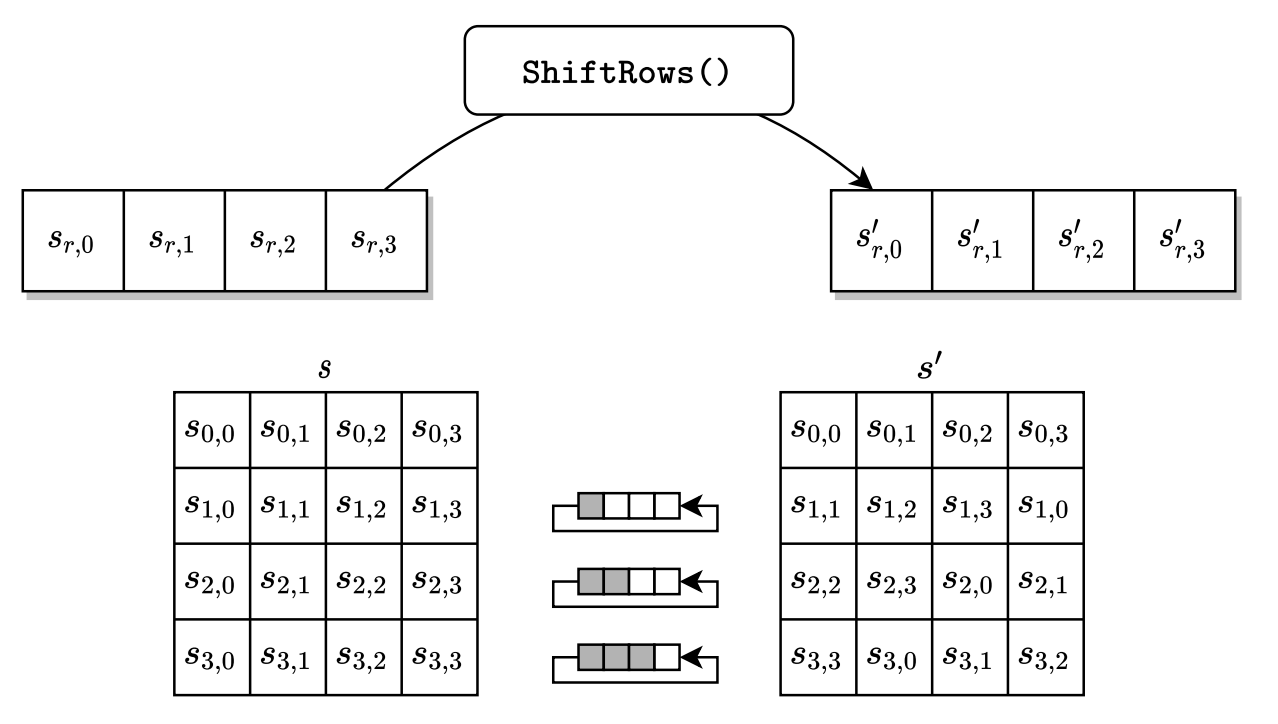
\includegraphics[width=0.85\linewidth]{images/ShiftRows.png}\par
\raggedright\scriptsize
\begin{itemize}
\item In flat indices ($s_{r,c}=\texttt{state}[r{+}4c]$) row 1 is a 4-cycle, row 2 swaps $2\!\leftrightarrow\!10$, $6\!\leftrightarrow\!14$, row 3 is a 4-cycle the other way.
\item Diffusion: the 4 bytes of a column go to 4 columns.
\end{itemize}
\end{column}
\begin{column}{0.43\textwidth}
\codesmall
%CODE utils.c
\begin{tbox}{utils.c :: ShiftRows}
\begin{lstlisting}
void ShiftRows(u8* state) {
    // Shift second row
    u8 temp = state[1];
    state[1]  = state[5];
    state[5]  = state[9];
    state[9]  = state[13];
    state[13] = temp;

    // Shift third row
    temp = state[2];
    state[2]  = state[10];
    state[10] = temp;
    temp = state[6];
    state[6]  = state[14];
    state[14] = temp;

    // Shift fourth row
    temp = state[15];
    state[15] = state[11];
    state[11] = state[7];
    state[7]  = state[3];
    state[3]  = temp;
}
\end{lstlisting}
\end{tbox}
\codenormal
\end{column}
\end{columns}
\src{FIPS 197 \S5.1.2, Eq.~5.5, Fig.~3; AESFINAL/utils.c}
\end{frame}

\begin{frame}{MixColumns: specification}
\begin{columns}[T]
\begin{column}{0.60\textwidth}
\small
Every column of the state is multiplied by a fixed matrix over $\GF$:
\[\setlength{\arraycolsep}{3pt}
\begin{bmatrix}s'_{0,c}\\s'_{1,c}\\s'_{2,c}\\s'_{3,c}\end{bmatrix}=
\begin{bmatrix}\hh{02}&\hh{03}&\hh{01}&\hh{01}\\\hh{01}&\hh{02}&\hh{03}&\hh{01}\\
\hh{01}&\hh{01}&\hh{02}&\hh{03}\\\hh{03}&\hh{01}&\hh{01}&\hh{02}\end{bmatrix}
\begin{bmatrix}s_{0,c}\\s_{1,c}\\s_{2,c}\\s_{3,c}\end{bmatrix},\quad 0\le c<4\]
\footnotesize
\begin{align*}
s'_{0,c}&=(\hx{02}\gm s_{0,c})\xor(\hx{03}\gm s_{1,c})\xor s_{2,c}\xor s_{3,c}\\
s'_{1,c}&=s_{0,c}\xor(\hx{02}\gm s_{1,c})\xor(\hx{03}\gm s_{2,c})\xor s_{3,c}\\
s'_{2,c}&=s_{0,c}\xor s_{1,c}\xor(\hx{02}\gm s_{2,c})\xor(\hx{03}\gm s_{3,c})\\
s'_{3,c}&=(\hx{03}\gm s_{0,c})\xor s_{1,c}\xor s_{2,c}\xor(\hx{02}\gm s_{3,c})
\end{align*}
\end{column}
\begin{column}{0.37\textwidth}
\centering
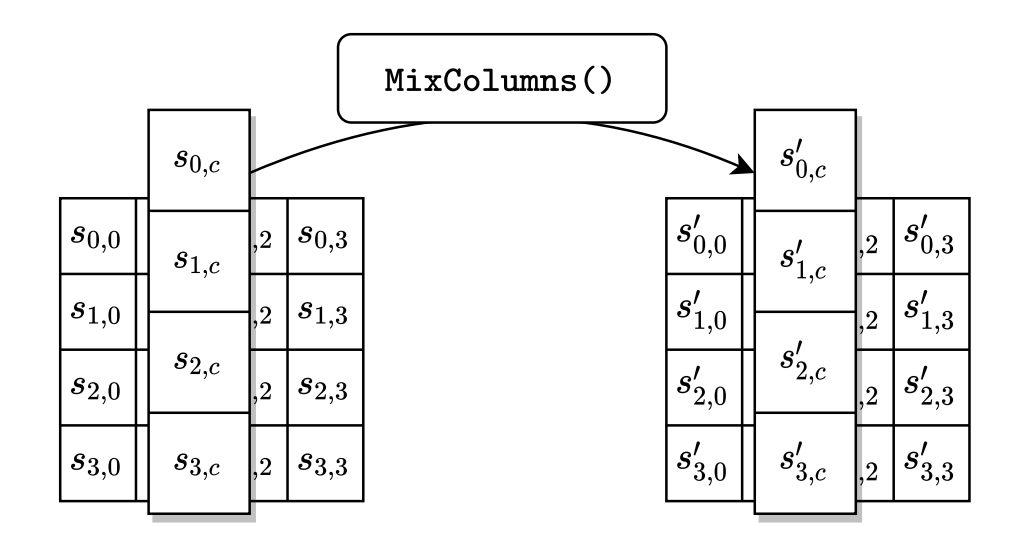
\includegraphics[width=\linewidth]{images/MixColumns.png}\par\vskip6pt
\raggedright\footnotesize
\begin{itemize}
\item Circulant matrix; first column $[\hx{02},\hx{01},\hx{01},\hx{03}]$; coefficients are cheap on 8-bit CPUs.
\item With ShiftRows it gives \alert{diffusion}: one input byte affects 4 output bytes.
\end{itemize}
\end{column}
\end{columns}
\src{FIPS 197 \S4.3, \S5.1.3 (Eq.~5.6--5.8), Fig.~4}
\end{frame}

\begin{frame}[fragile]{MixColumns: efficient evaluation with xtime}
\begin{columns}[T]
\begin{column}{0.52\textwidth}
\small
For a column $[a_0,a_1,a_2,a_3]$ let $t=a_0\xor a_1\xor a_2\xor a_3$.
Then, with indices mod 4,
\[ a'_i=a_i\xor\fn{xtime}(a_i\xor a_{i+1})\xor t. \]
\footnotesize
Check for $i=0$ (using $\hx{03}\gm a=\hx{02}\gm a\xor a$):
\begin{align*}
a_0\xor\hx{02}\gm(a_0\xor a_1)\xor t
&=\hx{02}\gm a_0\xor\hx{02}\gm a_1\xor a_1\xor a_2\xor a_3\\
&=\hx{02}\gm a_0\xor\hx{03}\gm a_1\xor a_2\xor a_3 .
\end{align*}
\begin{itemize}
\item The \alert{only} field multiplication is $\fn{xtime}$.
\item Per column: 1 four-way XOR, 4 xtime, 8 XOR.
\end{itemize}
\end{column}
\begin{column}{0.45\textwidth}
%CODE utils.c
\begin{tbox}{utils.c :: MixColumns (column 0)}
\begin{lstlisting}
void MixColumns(u8* s) {
    // Mix first column
    u8 t = s[0] ^ s[1] ^ s[2] ^ s[3];
    u8 temp = s[0];
    s[0] ^= xtime(s[0] ^ s[1]) ^ t;
    s[1] ^= xtime(s[1] ^ s[2]) ^ t;
    s[2] ^= xtime(s[2] ^ s[3]) ^ t;
    s[3] ^= xtime(s[3] ^ temp) ^ t;
    ...
    // Mix fourth column
    t = s[12] ^ s[13] ^ s[14] ^ s[15];
    temp = s[12];
    s[12] ^= xtime(s[12] ^ s[13]) ^ t;
    ...
    s[15] ^= xtime(s[15] ^ temp)  ^ t;
}
\end{lstlisting}
\end{tbox}
\vskip3pt
{\footnotesize \texttt{temp} keeps the old $a_0$, needed for $a'_3$ after $a_0$ was overwritten.}
\end{column}
\end{columns}
\src{FIPS 197 \S5.1.3; Rijndael AES Implementation \S3.3; AESFINAL/utils.c}
\end{frame}

\begin{frame}[fragile]{AddRoundKey}
\begin{columns}[T]
\begin{column}{0.56\textwidth}
\footnotesize
The round key (4 words of the key schedule) is XORed into the 4 columns:
\[ [s'_{0,c},s'_{1,c},s'_{2,c},s'_{3,c}]=[s_{0,c},s_{1,c},s_{2,c},s_{3,c}]\xor w[4\cdot\mathit{round}+c] \]
for $0\le c<4$ and $0\le\mathit{round}\le\Nr$.\\[3pt]
\centering
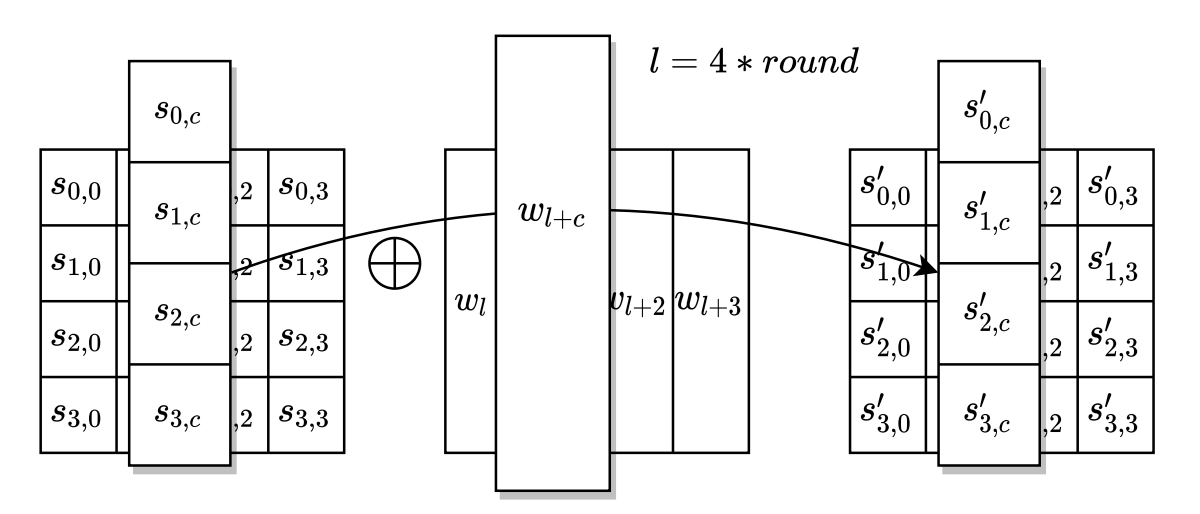
\includegraphics[width=0.9\linewidth]{images/Round.png}\par
\raggedright\scriptsize
\begin{itemize}
\item In the figure $l=4\cdot\mathit{round}$. Self-inverse: $(s\xor k)\xor k=s$.
\item One 128-bit XOR handles all 16 bytes: \alert{SIMD (SSE2)}.
\end{itemize}
\end{column}
\begin{column}{0.41\textwidth}
\codesmall
%CODE utils.c
\begin{tbox}{utils.c :: AddRoundKey}
\begin{lstlisting}
void AddRoundKey(u8* state, u8* ExpandedKey,
                 u8 round) {
    // Load 16 bytes from the state and
    // the corresponding round key
    __m128i* stateVec = (__m128i*)state;
    __m128i* roundKeyVec =
        (__m128i*)(ExpandedKey + 16 * round);

    // XOR 16 bytes at once
    *stateVec = _mm_xor_si128(*stateVec,
                              *roundKeyVec);
}
\end{lstlisting}
\end{tbox}
\codenormal
\vskip3pt
{\footnotesize Round key $\mathit{round}$ starts at byte $16\cdot\mathit{round}$ of \texttt{ExpandedKey}.}
\end{column}
\end{columns}
\src{FIPS 197 \S5.1.4 (Eq.~5.9), Fig.~5; Rijndael AES Implementation \S3.4; AESFINAL/utils.c}
\end{frame}

\begin{frame}[fragile]{KeyExpansion: algorithm}
\begin{columns}[T]
\begin{column}{0.60\textwidth}
\footnotesize
\begin{pseudo}
1 & \texttt{KeyExpansion}($\mathit{key}$): $w[i]\leftarrow\mathit{key}[4i..4i{+}3]$, $0\le i<\Nk$ \\
2 & \kw{for} $i=\Nk$ \kw{to} $4\Nr+3$ \kw{do} \\
3 & \ind $\mathit{temp}\leftarrow w[i-1]$ \\
4 & \ind \kw{if} $i\bmod \Nk=0$ \kw{then} \\
5 & \ind\ind $\mathit{temp}\leftarrow\fn{SubWord}(\fn{RotWord}(\mathit{temp}))\xor\fn{Rcon}[i/\Nk]$ \\
6 & \ind \kw{else if} $\Nk>6$ \kw{and} $i\bmod\Nk=4$ \kw{then} \\
7 & \ind\ind $\mathit{temp}\leftarrow\fn{SubWord}(\mathit{temp})$ \\
8 & \ind $w[i]\leftarrow w[i-\Nk]\xor\mathit{temp}$ \\
\end{pseudo}
\vskip3pt
\begin{itemize}\footnotesize
\item $\fn{RotWord}([a_0,a_1,a_2,a_3])=[a_1,a_2,a_3,a_0]$
\item $\fn{SubWord}([a_0,\dots,a_3])=[\fn{SBox}(a_0),\dots,\fn{SBox}(a_3)]$
\item $\fn{Rcon}[j]=[x^{j-1},\hx{00},\hx{00},\hx{00}]$ in $\GF$, i.e.\ $x^{j-1}$ by repeated $\fn{xtime}$.
\item Lines 6--7 apply to AES-256 only; AES-128 uses $\Nk=4$.
\end{itemize}
\vskip2pt\scriptsize
AES-128, $l=0,4,\dots,36$: $w[l{+}4]=w[l]\xor\fn{SubWord}(\fn{RotWord}(w[l{+}3]))\xor\fn{Rcon}[\tfrac{l+4}{4}]$, and $w[l{+}k]=w[l{+}k{-}4]\xor w[l{+}k{-}1]$ for $k=5,6,7$.
\end{column}
\begin{column}{0.37\textwidth}
\footnotesize\centering
\begin{tabular}{@{}cc@{\hspace{6pt}}cc@{}}
\toprule
$j$ & $\fn{Rcon}[j]_0$ & $j$ & $\fn{Rcon}[j]_0$\\
\midrule
1&\hh{01}&6&\hh{20}\\ 2&\hh{02}&7&\hh{40}\\ 3&\hh{04}&8&\hh{80}\\
4&\hh{08}&9&\hh{1b}\\ 5&\hh{10}&10&\hh{36}\\
\bottomrule
\end{tabular}
\vskip5pt
\raggedright
%CODE utils.c
\begin{tbox}{utils.c :: Rcon}
\begin{lstlisting}
// AES round constants
const u8 Rcon[10] =
{0x01, 0x02, 0x04, 0x08, 0x10,
 0x20, 0x40, 0x80, 0x1B, 0x36};
\end{lstlisting}
\end{tbox}
{\footnotesize The array stores only the leftmost byte of each $\fn{Rcon}[j]$ (the other three are $\hx{00}$).}
\end{column}
\end{columns}
\src{FIPS 197 \S5.2, Alg.~2, Table 5; AESFINAL/utils.c}
\end{frame}

\begin{frame}[fragile]{KeyExpansion: AES-128 data flow and C}
\begin{columns}[T]
\begin{column}{0.30\textwidth}
\centering
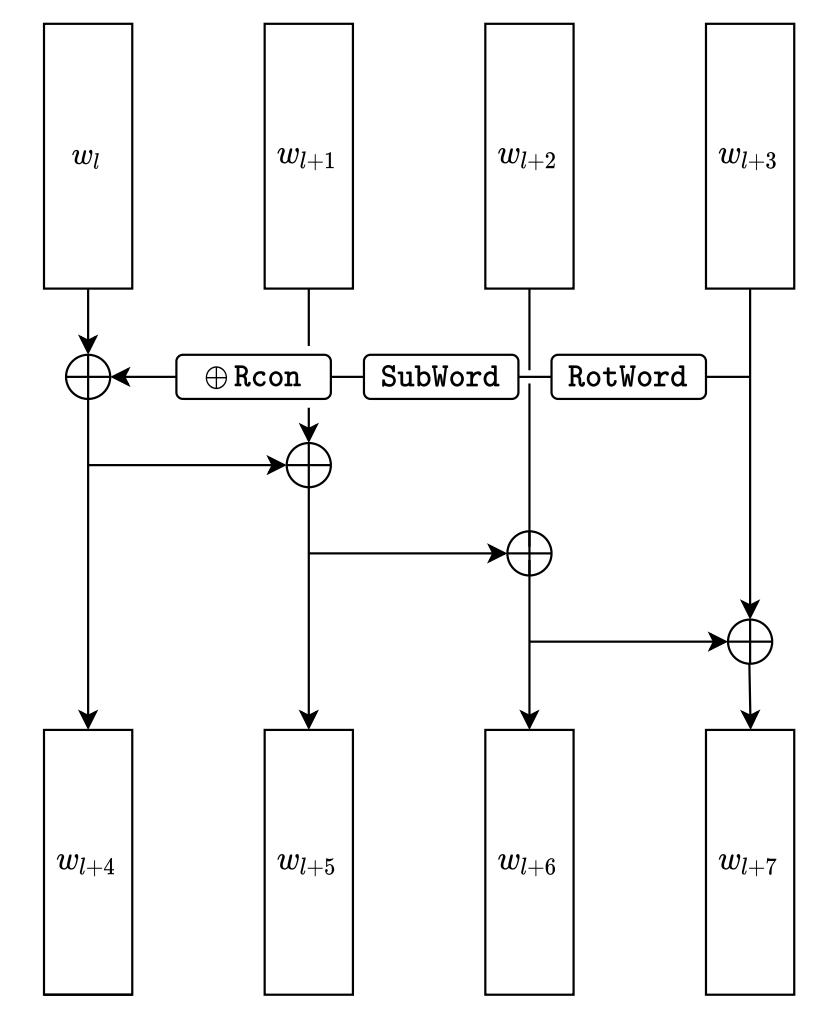
\includegraphics[height=60mm]{images/RoundKey.png}
\end{column}
\begin{column}{0.68\textwidth}
\footnotesize
New word $=$ word 4 earlier $\xor$ previous new word; the first also uses $\fn{RotWord}$, $\fn{SubWord}$, $\fn{Rcon}$.
\codesmall
%CODE utils.c
\begin{tbox}{utils.c :: KeyExpansion (AES-128)}
\begin{lstlisting}
void KeyExpansion(u8* key, u8* w) {
    u8 temp[4];
    for (int j = 0; j < 16; ++j)
        w[j] = key[j];
    for (int i = NK; i < 4 * (NR + 1); ++i) {
        temp[0] = w[4*(i-1)];
        temp[1] = w[4*(i-1) + 1];
        temp[2] = w[4*(i-1) + 2];
        temp[3] = w[4*(i-1) + 3];
        if (i % NK == 0) {  // RotWord + SubWord + Rcon
            u8 t = temp[0];
            temp[0] = sbox[temp[1]] ^ Rcon[(i/NK) - 1];
            temp[1] = sbox[temp[2]];
            temp[2] = sbox[temp[3]];
            temp[3] = sbox[t];
        }
        w[4*i]     = w[4*(i-NK)]     ^ temp[0];
        w[4*i + 1] = w[4*(i-NK) + 1] ^ temp[1];
        w[4*i + 2] = w[4*(i-NK) + 2] ^ temp[2];
        w[4*i + 3] = w[4*(i-NK) + 3] ^ temp[3];
    }
}
\end{lstlisting}
\end{tbox}
\codenormal
\end{column}
\end{columns}
\src{FIPS 197 Fig.~6; Rijndael AES Implementation \S3.5; AESFINAL/utils.c}
\end{frame}

% ============================================================
\section{DECRYPTION}

\begin{frame}[fragile]{InvCipher()}
\begin{columns}[T]
\begin{column}{0.52\textwidth}
\small
Invert every transformation and run them in \alert{reverse order}:\par\vskip3pt
\begin{pseudo}
1 & \kw{procedure} \texttt{InvCipher}($\mathit{in},\Nr,w$) \\
2 & \ind $\mathit{state}\leftarrow\fn{AddRoundKey}(\mathit{in},w[4\Nr..4\Nr{+}3])$ \\
3 & \ind \kw{for} $\mathit{round}=\Nr-1$ \kw{downto} $1$ \kw{do} \\
4 & \ind\ind $\fn{InvShiftRows}$ \\
5 & \ind\ind $\fn{InvSubBytes}$ \\
6 & \ind\ind $\fn{AddRoundKey}(\cdot,w[4\,\mathit{round}..4\,\mathit{round}{+}3])$ \\
7 & \ind\ind $\fn{InvMixColumns}$ \\
8 & \ind $\fn{InvShiftRows};\ \fn{InvSubBytes}$ \\
9 & \ind $\fn{AddRoundKey}(\cdot,w[0..3])$ \\
\end{pseudo}
\vskip3pt
\footnotesize
$\fn{AddRoundKey}$ is its own inverse. Decryption keeps the encryption
key schedule $w$ and uses the round keys in reverse order.
\end{column}
\begin{column}{0.45\textwidth}
%CODE utils.c
\begin{tbox}{utils.c :: InvCipher}
\begin{lstlisting}
void InvCipher( u8* state, u8* ExpandedKey) {
    AddRoundKey(state, ExpandedKey, 10);

    for (u8 round = NR-1; round > 0; round--) {
        InvShiftRows(state);
        InvSubBytes(state);
        AddRoundKey(state, ExpandedKey, round);
        InvMixColumns(state);
    }

    InvShiftRows(state);
    InvSubBytes(state);
    AddRoundKey(state, ExpandedKey, 0);
}
\end{lstlisting}
\end{tbox}
\vskip3pt
{\footnotesize This is the function called by \texttt{ecb\_decrypt} and \texttt{cbc\_decrypt}.}
\end{column}
\end{columns}
\src{FIPS 197 \S5.3, Alg.~3; Rijndael AES Implementation \S4; AESFINAL/utils.c}
\end{frame}

\begin{frame}[fragile]{InvShiftRows}
\begin{columns}[T]
\begin{column}{0.54\textwidth}
\small
Row $r$ is cyclically shifted \alert{right} by $r$ bytes:
\[ s'_{r,c}=s_{r,(c-r)\bmod 4},\qquad 0\le r,c<4 \]
\centering
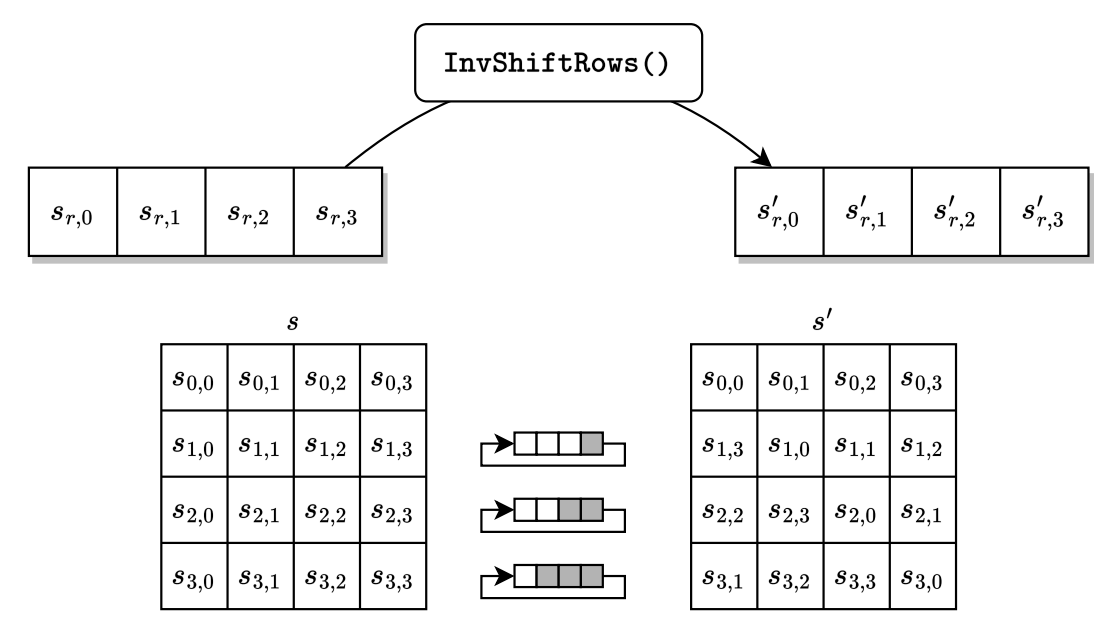
\includegraphics[width=0.85\linewidth]{images/InvShiftRows.png}\par
\raggedright\scriptsize
\begin{itemize}
\item $\fn{ShiftRows}$ maps column $c$ to $c-r$ and $\fn{InvShiftRows}$ maps it back: $(c-r)+r\equiv c \pmod 4$.
\item Row 2 is self-inverse: shifting by $2$ and by $-2$ coincide mod 4.
\end{itemize}
\end{column}
\begin{column}{0.43\textwidth}
\codesmall
%CODE utils.c
\begin{tbox}{utils.c :: InvShiftRows}
\begin{lstlisting}
void InvShiftRows(u8* state) {
    // Shift back second row
    u8 temp = state[13];
    state[13] = state[9];
    state[9] = state[5];
    state[5] = state[1];
    state[1] = temp;

    // Shift back third row
    temp = state[2];
    state[2] = state[10];
    state[10] = temp;
    temp = state[6];
    state[6] = state[14];
    state[14] = temp;

    // Shift back fourth row
    temp = state[3];
    state[3] = state[7];
    state[7] = state[11];
    state[11] = state[15];
    state[15] = temp;
}
\end{lstlisting}
\end{tbox}
\codenormal
\end{column}
\end{columns}
\src{FIPS 197 \S5.3.1, Eq.~5.12, Fig.~9; AESFINAL/utils.c}
\end{frame}

\begin{frame}[fragile]{InvSubBytes}
\begin{columns}[T]
\begin{column}{0.54\textwidth}
\small
$\fn{InvSBox}$ is $\fn{SBox}$ with the roles of input and output swapped:
\[ \fn{InvSBox}(\fn{SBox}(b))=b,\qquad s'_{r,c}=\fn{InvSBox}(s_{r,c}) \]
\footnotesize
\begin{itemize}
\item Construction: $\fn{InvSBox}=g\circ f^{-1}$ (inverse affine map, then inversion in $\GF$).
\item Example: $\fn{SBox}(\hx{53})=\hx{ed}$ and $\fn{InvSBox}(\hx{ed})=\hx{53}$.
\item Implemented as a second 256-byte table, again with the loop unrolled.
\end{itemize}
\end{column}
\begin{column}{0.43\textwidth}
%CODE utils.c
\begin{tbox}{utils.c :: InvSbox, InvSubBytes}
\begin{lstlisting}
const u8 InvSbox[256]  = {
    0x52, 0x09, 0x6a, 0xd5, 0x30, 0x36,
    0xa5, 0x38, 0xbf, 0x40, 0xa3, 0x9e,
    ...
};
\end{lstlisting}
\vskip3pt
\begin{lstlisting}
void InvSubBytes(u8* state) {
    state[0]  = InvSbox[state[0]];
    state[1]  = InvSbox[state[1]];
    ...
    state[15] = InvSbox[state[15]];
}
\end{lstlisting}
\end{tbox}
\end{column}
\end{columns}
\src{FIPS 197 \S5.3.2, Table 6; Rijndael AES Implementation \S2.2; AESFINAL/utils.c}
\end{frame}

\begin{frame}[fragile]{InvMixColumns: Barreto's factorisation}
\footnotesize
\[\setlength{\arraycolsep}{2.5pt}
\underbrace{\begin{bmatrix}\hh{0e}&\hh{0b}&\hh{0d}&\hh{09}\\\hh{09}&\hh{0e}&\hh{0b}&\hh{0d}\\\hh{0d}&\hh{09}&\hh{0e}&\hh{0b}\\\hh{0b}&\hh{0d}&\hh{09}&\hh{0e}\end{bmatrix}}_{\text{InvMixColumns}}=
\underbrace{\begin{bmatrix}\hh{02}&\hh{03}&\hh{01}&\hh{01}\\\hh{01}&\hh{02}&\hh{03}&\hh{01}\\\hh{01}&\hh{01}&\hh{02}&\hh{03}\\\hh{03}&\hh{01}&\hh{01}&\hh{02}\end{bmatrix}}_{\text{MixColumns}}
\underbrace{\begin{bmatrix}\hh{05}&\hh{00}&\hh{04}&\hh{00}\\\hh{00}&\hh{05}&\hh{00}&\hh{04}\\\hh{04}&\hh{00}&\hh{05}&\hh{00}\\\hh{00}&\hh{04}&\hh{00}&\hh{05}\end{bmatrix}}_{P}\]
\vskip-4pt
\begin{columns}[T]
\begin{column}{0.54\textwidth}
\begin{itemize}
\item As polynomials: $d(x)=\big(\hx{04}x^2+\hx{05}\big)\otimes c(x)\bmod(x^4+\hx{01})$.
\item Direct coefficients $\hx{09},\hx{0b},\hx{0d},\hx{0e}$ need many $\fn{xtime}$ calls.
\item Instead: a cheap \alert{pre-processing} $P$, then the existing $\fn{MixColumns}$:
\[ u=\fn{xtime}^2(a_0\xor a_2),\quad v=\fn{xtime}^2(a_1\xor a_3) \]
\[ (a_0,a_1,a_2,a_3)\leftarrow(a_0\xor u,\ a_1\xor v,\ a_2\xor u,\ a_3\xor v) \]
\end{itemize}
\end{column}
\begin{column}{0.43\textwidth}
%CODE utils.c
\begin{tbox}{utils.c :: InvMixColumns}
\begin{lstlisting}
void InvMixColumns(u8* s) {
    u8 u = xtime(xtime(s[0] ^ s[2]));
    u8 v = xtime(xtime(s[1] ^ s[3]));
    s[0] ^= u;
    s[1] ^= v;
    s[2] ^= u;
    s[3] ^= v;
    ...  // same for columns 1, 2, 3
    MixColumns(s);
}
\end{lstlisting}
\end{tbox}
\end{column}
\end{columns}
\src{FIPS 197 \S5.3.3 (Eq.~5.13--5.15); Rijndael AES Implementation \S4, Eq.~(1) (P.~Barreto); AESFINAL/utils.c}
\end{frame}

\begin{frame}[fragile]{EqInvCipher and KeyExpansionEIC}
\begin{columns}[T]
\begin{column}{0.50\textwidth}
\footnotesize
Same \emph{order} as $\fn{Cipher}$, each step replaced by its inverse:\par\vskip2pt
\begin{pseudo}
1 & $\fn{AddRoundKey}(\mathit{in},dw[4\Nr..4\Nr{+}3])$ \\
2 & \kw{for} $\mathit{round}=\Nr-1$ \kw{downto} $1$ \kw{do} \\
3 & \ind $\fn{InvSubBytes};\ \fn{InvShiftRows}$ \\
4 & \ind $\fn{InvMixColumns}$ \\
5 & \ind $\fn{AddRoundKey}(\cdot,dw[4\,\mathit{round}..+3])$ \\
6 & $\fn{InvSubBytes};\ \fn{InvShiftRows}$ \\
7 & $\fn{AddRoundKey}(\cdot,dw[0..3])$ \\
\end{pseudo}
\vskip3pt
Key schedule $dw$: $dw[i]=w[i]$, except for $1\le\mathit{round}\le\Nr{-}1$:
\[ dw[4\mathit{round}..{+}3]\leftarrow\fn{InvMixColumns}\big(w[4\mathit{round}..{+}3]\big) \]
\textbf{Why equivalent:} $\fn{InvSubBytes}$ and $\fn{InvShiftRows}$ commute, and
$\fn{InvMixColumns}$ is linear, so $\fn{InvMix}(s\xor k)=\fn{InvMix}(s)\xor\fn{InvMix}(k)$.
\end{column}
\begin{column}{0.47\textwidth}
%CODE utils.c
\begin{tbox}{utils.c :: EqInvCipher}
\begin{lstlisting}
void EqInvCipher(u8* state, u8* ExpandedKey) {
    AddRoundKey(state, ExpandedKey, 10);
    for (u8 round = NR-1; round > 0; round--) {
        InvSubBytes(state);
        InvShiftRows(state);
        InvMixColumns(state);
        AddRoundKey(state, ExpandedKey, round);
    }
    InvSubBytes(state);
    InvShiftRows(state);
    AddRoundKey(state, ExpandedKey, 0);
}
\end{lstlisting}
\end{tbox}
\vskip3pt
%CODE utils.c
\begin{tbox}{utils.c :: KeyExpansionEIC (tail)}
\begin{lstlisting}
    // Apply InvMixColumns to the key schedule
    for (int round = 1; round < NR; ++round) {
        int i = 16 * round;
        InvMixColumns(dw+i);
    }
\end{lstlisting}
\end{tbox}
\end{column}
\end{columns}
\src{FIPS 197 \S5.3.5, Alg.~4--5; Rijndael AES Implementation \S4; AESFINAL/utils.c}
\end{frame}

% ============================================================
\section{LOOK-UP TABLES}

\begin{frame}{From round to T-tables (1/2)}
\small
Let $a$ be the round input, $b$ the output of SubBytes, $c$ of ShiftRows, $d$ of MixColumns
($0\le j<\Nb$, shift offsets $C_i$, indices mod $\Nb$):
\begin{align*}
b_{i,j}&=\fn{SBox}[a_{i,j}], &
c_{i,j}&=b_{i,\,j+C_i}, &
\begin{bmatrix}d_{0,j}\\d_{1,j}\\d_{2,j}\\d_{3,j}\end{bmatrix}&=
\begin{bmatrix}\hh{02}&\hh{03}&\hh{01}&\hh{01}\\\hh{01}&\hh{02}&\hh{03}&\hh{01}\\\hh{01}&\hh{01}&\hh{02}&\hh{03}\\\hh{03}&\hh{01}&\hh{01}&\hh{02}\end{bmatrix}
\begin{bmatrix}c_{0,j}\\c_{1,j}\\c_{2,j}\\c_{3,j}\end{bmatrix}
\end{align*}
Substitute and read the matrix product as a combination of its \alert{four columns}:
{\footnotesize\setlength{\arraycolsep}{2pt}
\[
\begin{bmatrix}d_{0,j}\\d_{1,j}\\d_{2,j}\\d_{3,j}\end{bmatrix}=
\begin{bmatrix}\hh{02}\\\hh{01}\\\hh{01}\\\hh{03}\end{bmatrix}\!\gm\fn{SBox}[a_{0,j+C_0}]\ \xor\
\begin{bmatrix}\hh{03}\\\hh{02}\\\hh{01}\\\hh{01}\end{bmatrix}\!\gm\fn{SBox}[a_{1,j+C_1}]\ \xor\
\begin{bmatrix}\hh{01}\\\hh{03}\\\hh{02}\\\hh{01}\end{bmatrix}\!\gm\fn{SBox}[a_{2,j+C_2}]\ \xor\
\begin{bmatrix}\hh{01}\\\hh{01}\\\hh{03}\\\hh{02}\end{bmatrix}\!\gm\fn{SBox}[a_{3,j+C_3}]
\]}
\vskip2pt
\footnotesize
The input to each term is a \emph{single byte}, so each term can be pre-computed for all 256 values.
\src{Rijndael AES Implementation \S5.1, Eq.~(1)--(5)}
\end{frame}

\begin{frame}{From round to T-tables (2/2)}
\begin{columns}[T]
\begin{column}{0.56\textwidth}
\footnotesize
Four tables of 256 four-byte words ($\fn{S}=\fn{SBox}$):
\begin{align*}
T_0[a]&=[\hh{02}\gm\fn{S}[a],\ \fn{S}[a],\ \fn{S}[a],\ \hh{03}\gm\fn{S}[a]]^{T}\\
T_1[a]&=[\hh{03}\gm\fn{S}[a],\ \hh{02}\gm\fn{S}[a],\ \fn{S}[a],\ \fn{S}[a]]^{T}\\
T_2[a]&=[\fn{S}[a],\ \hh{03}\gm\fn{S}[a],\ \hh{02}\gm\fn{S}[a],\ \fn{S}[a]]^{T}\\
T_3[a]&=[\fn{S}[a],\ \fn{S}[a],\ \hh{03}\gm\fn{S}[a],\ \hh{02}\gm\fn{S}[a]]^{T}
\end{align*}
One round, column $j$, \emph{including} AddRoundKey:
\[\begin{aligned}[]
[d_{0,j},\dots,d_{3,j}]^{T}={}&T_0[a_{0,j+C_0}]\xor T_1[a_{1,j+C_1}]\xor T_2[a_{2,j+C_2}]\\
&\xor T_3[a_{3,j+C_3}]\xor w[4\,\mathit{round}+j]\end{aligned}\]
\end{column}
\begin{column}{0.41\textwidth}
\begin{tbox}{cost and trade-offs}
\footnotesize
\begin{itemize}
\item 4 look-ups + 4 XORs per column per round, for 32-bit or wider words.
\item $4\times256\times4$ bytes $=$ \alert{4 kB} of tables ($T_k$ are byte-rotations of $T_0$).
\item The final round has no MixColumns and uses plain $\fn{SBox}$.
\item Secret-dependent table indices make \alert{cache-timing attacks} possible (Osvik--Shamir--Tromer).
\end{itemize}
\end{tbox}
\vskip4pt
\footnotesize
AESFINAL does \emph{not} use T-tables: it keeps the compact $\fn{SubBytes}$/$\fn{MixColumns}$ code
with a 256-byte S-box.
\end{column}
\end{columns}
\src{Rijndael AES Implementation \S5.1; Osvik, Shamir, Tromer, J.\ Cryptology 23 (2010)}
\end{frame}

% ============================================================
\section{MODES OF OPERATION}

\begin{frame}[fragile]{Modes of operation: IV and padding}
\begin{columns}[T]
\begin{column}{0.52\textwidth}
\small
A message $m=m_0m_1\dots$ is processed in 128-bit blocks; the mode defines how
$E_K$ is used (NIST SP 800-38A).
\begin{itemize}\footnotesize
\item \alert{IV}: a block-sized value for CBC, OFB (and CFB); a nonce for CTR.
  We draw it with OpenSSL \texttt{RAND\_bytes} and store it as the first 16 bytes of the file.
\item ECB and CBC need whole blocks: \alert{PKCS\#7 padding}. If the last block has $\ell$ bytes ($0\le\ell<16$), append $p=16-\ell$ bytes each of value $p$ (so $1\le p\le16$; a full block of padding is added when $\ell=0$).
\item Decryption reads the last byte $p$, checks that the last $p$ bytes equal $p$, and removes them.
\end{itemize}
\vskip2pt
{\footnotesize Modes covered: ECB, CBC, OFB, CTR (CFB is implemented in the code but not presented).}
\end{column}
\begin{column}{0.45\textwidth}
\codesmall
%CODE moops.c
\begin{tbox}{moops.c :: IV and padding}
\begin{lstlisting}
unsigned char IV[16];

void generate_iv() {
    if (!RAND_bytes(IV, sizeof(IV))) {
        perror("Error generating random IV");
        exit(EXIT_FAILURE);
    }
}
...
u8 pkcs7_unpad(u8* plaintext) {
    u8 pad_value = plaintext[15];
    if (pad_value > 0 && pad_value <= 16) {
        for (u8 i = 0; i < pad_value; ++i) {
            if (plaintext[16 - 1 - i] != pad_value) {
                ...
            }
        }
        return pad_value;
    } else {
        ...
    }
}
\end{lstlisting}
\end{tbox}
\codenormal
\end{column}
\end{columns}
\src{Rijndael AES Implementation \S6; NIST SP 800-38A; Kaliski, RFC 2315; AESFINAL/moops.c}
\end{frame}

\begin{frame}[fragile]{ECB: electronic codebook}
\begin{columns}[T]
\begin{column}{0.48\textwidth}
\footnotesize
\textbf{Encryption:}\quad $c_i=E_K(m_i)$\\[2pt]
\textbf{Decryption:}\quad $m_i=D_K(c_i)$
\end{column}
\begin{column}{0.48\textwidth}
\footnotesize
\alert{Weakness}: $m_i=m_j\Rightarrow c_i=c_j$. Patterns of a low-entropy plaintext
space survive encryption; ECB is virtually never used in practice.
\end{column}
\end{columns}
\vskip4pt
\codesmall
\begin{columns}[T]
\begin{column}{0.49\textwidth}
%CODE moops.c
\begin{tbox}{moops.c :: ecb\_encrypt}
\begin{lstlisting}
void ecb_encrypt(FILE* ifile, FILE *ofile, u8* ExpandedKey){
    u8 in_block[16];
    u8 bytes_read;
    while ((bytes_read = fread(in_block, 1, 16, ifile)) == 16) {
        Cipher(in_block, ExpandedKey);
        fwrite(in_block, 1, 16, ofile);
    }
    // Apply PKCS#7 padding
    u8 padding_value = 16 - bytes_read;
    for (u8 i = bytes_read; i < 16; ++i)
        in_block[i] = padding_value;
    Cipher(in_block, ExpandedKey);
    fwrite(in_block, 1, 16, ofile);
}
\end{lstlisting}
\end{tbox}
\end{column}
\begin{column}{0.49\textwidth}
%CODE moops.c
\begin{tbox}{moops.c :: ecb\_decrypt}
\begin{lstlisting}
void ecb_decrypt(FILE* ifile, FILE *ofile, u8* ExpandedKey){
    u8 in_block[16], out_block[16];
    u8 bytes_read;
    while (fread(in_block, 1, 16, ifile) > 0) {
        InvCipher(in_block, ExpandedKey);
        fwrite(in_block, 1, 16, ofile);
    }
    // Handle the last block with padding removal
    u8 pad_len = pkcs7_unpad(in_block);
    fseek(ofile, -pad_len,SEEK_END);
    long current_pos = ftell(ofile);
    ftruncate(fileno(ofile), current_pos);
}
\end{lstlisting}
\end{tbox}
\end{column}
\end{columns}
\codenormal
\src{Rijndael AES Implementation \S6.1; AESFINAL/moops.c}
\end{frame}

\begin{frame}[fragile]{CBC: cipher block chaining}
\begin{columns}[T]
\begin{column}{0.48\textwidth}
\footnotesize
\textbf{Encryption:}
$\begin{cases}c_0=E_K(m_0\xor IV)\\ c_i=E_K(m_i\xor c_{i-1}),\ i\ge1\end{cases}$
\end{column}
\begin{column}{0.48\textwidth}
\footnotesize
\textbf{Decryption:}
$\begin{cases}m_0=D_K(c_0)\xor IV\\ m_i=D_K(c_i)\xor c_{i-1},\ i\ge1\end{cases}$
\end{column}
\end{columns}
\vskip2pt
\footnotesize
Random IV $\Rightarrow$ CPA-secure (CCA needs authenticated encryption). Encryption is sequential; decryption is parallelisable ($m_i$ needs only $c_i,c_{i-1}$).
\vskip3pt
\codesmall
\begin{columns}[T]
\begin{column}{0.49\textwidth}
%CODE moops.c
\begin{tbox}{moops.c :: cbc\_encrypt}
\begin{lstlisting}
void cbc_encrypt(FILE* ifile, FILE *ofile, u8* ExpandedKey){
    u8 plaintext[16];
    u8 bytes_read;
    generate_iv();
    fwrite(IV, 1, 16, ofile);
    while ((bytes_read = fread(plaintext, 1, 16, ifile)) == 16) {
        for (u8 i = 0; i < 16; ++i)
            IV[i] ^= plaintext[i] ;
        Cipher(IV, ExpandedKey);
        fwrite(IV, 1, 16, ofile);
    }
    ... // last block: PKCS#7 pad, XOR with IV,
    ... // Cipher, write (same chaining)
}
\end{lstlisting}
\end{tbox}
\end{column}
\begin{column}{0.49\textwidth}
%CODE moops.c
\begin{tbox}{moops.c :: cbc\_decrypt}
\begin{lstlisting}
void cbc_decrypt(FILE* ifile, FILE *ofile, u8* ExpandedKey){
    u8 input[16], temp[16], output[16];
    u8 bytes_read;
    fread(IV, 1, 16, ifile);
    while (fread(input, 1, 16, ifile) > 0) {
        for (u8 i = 0; i < 16; i++)
            temp[i] = input[i];
        InvCipher(input, ExpandedKey);
        for (u8 i = 0; i < 16; ++i)
            input[i] ^= IV[i];
        for (u8 i = 0; i < 16; i++)
            IV[i] = temp[i];
        fwrite(input, 1, 16, ofile);
    }
    ... // unpad last block, truncate file
}
\end{lstlisting}
\end{tbox}
\end{column}
\end{columns}
\codenormal
\src{Rijndael AES Implementation \S6.2; AESFINAL/moops.c. Global \texttt{IV} is the chaining register.}
\end{frame}

\begin{frame}[fragile]{OFB: output feedback}
\begin{columns}[T]
\begin{column}{0.46\textwidth}
\small
Synchronous stream cipher: the keystream is the iterated encryption of the IV.
\[ \begin{cases} z_0=IV\\ z_i=E_K(z_{i-1}),\ i\ge1\\ c_i=z_i\xor m_i\end{cases} \]
Decryption is identical: $m_i=z_i\xor c_i$.
\begin{itemize}\footnotesize
\item $E_K$ is used for \alert{both} directions; $D_K$ is never needed.
\item No padding: the last partial block is simply truncated.
\item Keystream independent of the data (can be pre-computed), but strictly sequential.
\item No security against CCA (Rogaway); never reuse $(K,IV)$.
\end{itemize}
\end{column}
\begin{column}{0.51\textwidth}
%CODE moops.c
\begin{tbox}{moops.c :: ofb (encrypt and decrypt)}
\begin{lstlisting}
void ofb(FILE* ifile, FILE *ofile, u8* ExpandedKey,
         char choice){
    u8 in_block[16];
    u8 bytes_read;
    generate_iv();
    if(choice == 'e') fwrite(IV, 1, 16, ofile);
    else fread(IV, 1, 16, ifile);

    while ((bytes_read = fread(in_block, 1, 16, ifile)) > 0) {
        Cipher(IV, ExpandedKey);
        xor(in_block,IV);
        fwrite(in_block, 1, bytes_read, ofile);
    }
}
\end{lstlisting}
\end{tbox}
\vskip3pt
{\footnotesize \texttt{Cipher(IV,\dots)} turns $z_{i-1}$ into $z_i$ in place; \texttt{xor} gives $c_i=z_i\xor m_i$. \texttt{choice} selects write or read of the IV.}
\end{column}
\end{columns}
\src{Rijndael AES Implementation \S6.4; AESFINAL/moops.c}
\end{frame}

\begin{frame}[fragile]{CTR: counter mode}
\begin{columns}[T]
\begin{column}{0.46\textwidth}
\small
Keystream from encrypting successive counter values ($\ell=128$):
\[ \begin{cases} T_i=(ctr+i-1)\bmod 2^{\ell}\\ c_i=E_K(T_i)\xor m_i,\ i\ge1\end{cases} \]
Decryption: $m_i=E_K(T_i)\xor c_i$.
\begin{itemize}\footnotesize
\item $ctr$ = 96-bit non-repeating nonce $\Vert$ 32-bit block counter, starting at 0.
\item Blocks are independent: \alert{parallel} encryption and decryption, pre-processing, random access.
\item Software and hardware efficient; marked as the best choice among the modes in Rijndael AES Implementation.
\item Never reuse a $(K,\text{nonce})$ pair.
\end{itemize}
\end{column}
\begin{column}{0.51\textwidth}
%CODE moops.c
\begin{tbox}{moops.c :: ctr (encrypt and decrypt)}
\begin{lstlisting}
void ctr(FILE *ifile, FILE *ofile, u8* ExpandedKey,
         char choice){
    generate_iv();
    if(choice == 'e') fwrite(IV, 1, 16, ofile);
    else fread(IV, 1, 16, ifile);
    IV[0]=IV[1]=IV[2]=IV[3]=0x00;
    u8 input[16], in_block[16];
    u8 bytes_read;
    while ((bytes_read = fread(in_block, 1, 16, ifile)) > 0) {
        for (u8 i = 0; i < 16; i++)
            input[i]=IV[i];
        Cipher(input,ExpandedKey);
        xor(in_block, input);
        fwrite(in_block, 1, bytes_read, ofile);
        for (u8 i = 0; i < 4; ++i)
            if (++IV[i] != 0) break;
    }
}
\end{lstlisting}
\end{tbox}
\end{column}
\end{columns}
\src{Rijndael AES Implementation \S6.5; AESFINAL/moops.c (\texttt{xor} operands swapped vs.\ original: see notes); counter in \texttt{IV[0..3]}}
\end{frame}

\begin{frame}{Modes: comparison}
\centering\footnotesize
\renewcommand{\arraystretch}{1.25}
\begin{tabular}{@{}lcccccc@{}}
\toprule
mode & uses & padding & IV / nonce & par.\ enc. & par.\ dec. & keystream pre-computable \\
\midrule
ECB & $E_K$ / $D_K$ & yes & none & yes & yes & -- \\
CBC & $E_K$ / $D_K$ & yes & random IV & no & yes & -- \\
OFB & $E_K$ only & no & unique IV & no & no & yes \\
CTR & $E_K$ only & no & unique nonce & yes & yes & yes \\
\bottomrule
\end{tabular}
\vskip8pt
\raggedright
\begin{itemize}
\item ECB leaks equality of blocks; CBC/OFB/CTR hide it when the IV is fresh.
\item None of the confidentiality modes authenticates the data: use authenticated encryption against active attackers.
\end{itemize}
\src{Rijndael AES Implementation \S6; NIST SP 800-38A}
\end{frame}

% ============================================================
\section{IMPLEMENTATION}

\begin{frame}[fragile]{Our implementation: driver and usage}
\begin{columns}[T]
\begin{column}{0.48\textwidth}
\begin{tbox}{AESFINAL/ layout}
\footnotesize
\begin{tabular}{@{}l@{\ }p{3.6cm}@{}}
\texttt{AES.c} & command-line driver \\
\texttt{utils.c/h} & S-box, round steps, key expansion, \texttt{Cipher}, \texttt{InvCipher} \\
\texttt{moops.c/h} & ECB, CBC, CFB, OFB, CTR; IV; PKCS\#7 \\
\end{tabular}
\end{tbox}
\vskip4pt
\begin{tbox}{build and run (readme.txt)}
\footnotesize\ttfamily
gcc -c utils.c\\
gcc -c moops.c\\
gcc -o AES AES.c utils.o moops.o -lcrypto\\[3pt]
./AES e 1 test.pdf out.pdf KEY16CHARS...\\
\ \ <op> <mode> <in> <out> <key>
\end{tbox}
\vskip2pt
{\scriptsize \texttt{op}: e/d. \texttt{mode}: 1 ECB, 2 CBC, 3 CFB, 4 OFB, 5 CTR. Key: 16 chars.}
\end{column}
\begin{column}{0.49\textwidth}
\codesmall
%CODE AES.c
\begin{tbox}{AES.c :: main (excerpt)}
\begin{lstlisting}
int main(int argc, char* argv[]) {
    if (argc != 6) {
        print_usage(argv[0]);
        return 1;
    }
    ...
    u8 key[16];
    for (int i = 0; i < 16; i++)
        sscanf(&argv[5][i], "%c", &key[i]);
    ...
    u8 ExpandedKey[176];
    KeyExpansion(key, ExpandedKey);

    FILE *ifile = fopen(argv[3], "rb");
    FILE *ofile = fopen(argv[4], "wb");
    ...
    if (argv[1][0] == 'e') {
        switch (argv[2][0]) {
        case '1':
            ecb_encrypt(ifile, ofile, ExpandedKey);
            break;
        ...
        default:
            ctr(ifile, ofile, ExpandedKey, 'e');
\end{lstlisting}
\end{tbox}
\codenormal
\end{column}
\end{columns}
\src{AESFINAL/AES.c, readme.txt}
\end{frame}

\begin{frame}{References}
\scriptsize\setlength{\itemsep}{1.5pt}
\begin{itemize}
\item[{[1]}] NIST. \emph{Advanced Encryption Standard (AES)}, FIPS PUB 197-upd1, 26 Nov 2001 (updated 9 May 2023). \texttt{doi:10.6028/NIST.FIPS.197-upd1}. [AES\_Docs.pdf]
\item[{[2]}] \emph{Rijndael AES Implementation}.
\item[{[3]}] \emph{Advanced Encryption Standard}, Wikipedia. \texttt{en.wikipedia.org/wiki/Advanced\_Encryption\_Standard} (history slides).
\item[{[4]}] \emph{Advanced Encryption Standard process}, Wikipedia. \texttt{en.wikipedia.org/wiki/Advanced\_Encryption\_Standard\_process} (competition timeline, finalists).
\item[{[5]}] J.~Daemen, V.~Rijmen. \emph{The Design of Rijndael: AES -- The Advanced Encryption Standard}. Springer, 2002 (2nd ed.\ 2020).
\item[{[6]}] NIST. \emph{Recommendation for Block Cipher Modes of Operation}, SP 800-38A, 2001. \texttt{doi:10.6028/NIST.SP.800-38A}.
\item[{[7]}] B.~Kaliski. \emph{PKCS \#7: Cryptographic Message Syntax}, RFC 2315, 1998.
\item[{[8]}] D.~A.~Osvik, A.~Shamir, E.~Tromer. Efficient Cache Attacks on AES, and Countermeasures. \emph{J.\ Cryptology} 23 (2010), 37--71.
\item[{[9]}] P.~Rogaway. \emph{Evaluation of Some Blockcipher Modes of Operation}, 2011.
\item[{[10]}] S.~Gueron (Intel). \emph{Intel Advanced Encryption Standard (AES) New Instructions Set}, white paper, May 2010.
\item[{[11]}] J.~Nechvatal et al. \emph{Report on the Development of the AES}, J.\ Res.\ NIST 106 (2001). \texttt{doi:10.6028/jres.106.023}.
\end{itemize}
\end{frame}

{\setbeamercolor{background canvas}{bg=black}
\begin{frame}[plain,noframenumbering]
\color{white}
\begin{columns}[c]
\begin{column}{0.50\textwidth}
{\small > exit 0}\par\vskip10pt
{\fontsize{34}{40}\selectfont\bfseries Thank you\,\terminalcursor}\par\vskip14pt
{\small Questions?}
\end{column}
\begin{column}{0.46\textwidth}
\centering
{\small\bfseries > git clone}\par\vskip3pt

\includegraphics[width=0.62\linewidth]{images/qr_repo.png}\par\vskip3pt
{\scriptsize\texttt{https://github.com/0r-gh0/AES-Presentation}}\par
{\tiny slides, LaTeX source and C code}
\end{column}
\end{columns}
\end{frame}}

\end{document}
